\documentclass[12pt,a4paper]{report}

\usepackage[margin=1in]{geometry}
\usepackage{setspace}
\usepackage{array}
\usepackage{booktabs}
\usepackage{longtable}
\usepackage{tabularx}
\usepackage{enumitem}
\usepackage{graphicx}
\usepackage{float}
\usepackage{hyperref}
\usepackage{xcolor}
\usepackage{tikz}
\usetikzlibrary{arrows.meta, positioning, shapes.geometric, shapes.misc, fit, calc}
\usepackage{titlesec}
\usepackage{fancyhdr}
\usepackage{caption}

\hypersetup{
  colorlinks=true,
  linkcolor=blue!60!black,
  urlcolor=blue!50!black,
  citecolor=blue!50!black,
  pdftitle={Emergency Resource Allocator Project Report},
  pdfauthor={Team Name Placeholder}
}

\definecolor{accent}{HTML}{1F4E79}
\definecolor{accentlight}{HTML}{EAF2F8}
\definecolor{muted}{HTML}{5A6B7A}
\definecolor{panel}{HTML}{F7F9FC}

\titleformat{\chapter}{\normalfont\Huge\bfseries\color{accent}}{\thechapter}{1em}{}
\titleformat{\section}{\normalfont\Large\bfseries\color{accent}}{\thesection}{1em}{}
\titleformat{\subsection}{\normalfont\large\bfseries\color{accent}}{\thesubsection}{1em}{}
\setlength{\parskip}{0.65em}
\setlength{\parindent}{0pt}
\onehalfspacing
\pagestyle{fancy}
\fancyhf{}
\fancyhead[L]{Emergency Resource Allocator}
\fancyhead[R]{Project Report}
\fancyfoot[C]{\thepage}

\newcommand{\placeholderline}[1]{\textit{#1}}
\newcommand{\screenshotplaceholder}[1]{%
  \begin{center}
    \fbox{%
      \begin{minipage}[c][2.2in][c]{0.88\linewidth}
        \centering
        \vspace{0.15in}
        \textbf{Screenshot Placeholder}\\[0.5em]
        \placeholderline{#1}\\[0.5em]
        \placeholderline{Insert image here before final submission.}
      \end{minipage}
    }
  \end{center}
}

\newcommand{\coverfield}[2]{\renewcommand{\arraystretch}{1.25}\begin{tabularx}{0.88\textwidth}{>{\bfseries}l X}#1 & #2\end{tabularx}}

\begin{document}

\begin{titlepage}
  \begin{center}
    \vspace*{0.5cm}
    {\Large \textbf{[INSTITUTION / UNIVERSITY NAME]}}\\[0.3cm]
    {\large Department of [DEPARTMENT NAME]}\\[1.2cm]

    
\begin{tikzpicture}
      \draw[rounded corners=16pt, line width=1.5pt, color=accent] (0,0) rectangle (13.5,3.2);
      \node[align=center] at (6.75,2.2) {\Huge\bfseries Emergency Resource Allocator};
      \node[align=center, text=muted] at (6.75,1.25) {C++ Data Structures Project Report};
      \node[align=center, text=accent] at (6.75,0.55) {Heap \textbullet{} Hash Table \textbullet{} Queue \textbullet{} Linked List \textbullet{} BST \textbullet{} Graph};
    \end{tikzpicture}

    \vspace{1.1cm}
    {\Large \textbf{Project Report}}\\[0.7cm]

    \renewcommand{\arraystretch}{1.3}
    \begin{tabular}{>{\bfseries}p{4cm} p{8cm}}
      Project Name & Emergency Resource Allocator \\
      Course / Subject & [COURSE NAME / CODE] \\
      Instructor / Supervisor & [SUPERVISOR NAME] \\
      Semester / Session & [SEMESTER / SESSION] \\
      Submission Date & [DATE] \\
    \end{tabular}

    \vspace{0.9cm}
    \begin{tabular}{|p{12.2cm}|}
      \hline
      \textbf{Team Details (placeholders)} \\
      \hline
      Team Name: [TEAM NAME] \\ 
      Member 1: [NAME] - [ROLL / ID] \\ 
      Member 2: [NAME] - [ROLL / ID] \\ 
      Member 3: [NAME] - [ROLL / ID] \\ 
      Member 4: [NAME] - [ROLL / ID] \\ 
      \hline
    \end{tabular}

    \vfill
    {\large Prepared by: [YOUR NAME OR TEAM NAME]}\\[0.3cm]
    {\large \today}
  \end{center}
\end{titlepage}

\pagenumbering{roman}
\chapter*{Abstract}
The Emergency Resource Allocator is a C++ triage simulator designed to demonstrate core data-structure concepts in a realistic hospital or disaster-response setting. The project prioritizes emergencies using a max-heap, manages resources through a hash table, handles overflow cases with a queue, records system events in a dispatch history, and extends the base design with a linked-list patient registry, a BST-based ordered resource index, and graph-based route suggestions.

The final system includes both a console interface and a browser-based interface served by the C++ backend. This report documents the problem statement, design goals, implemented data structures, application architecture, algorithms, complexity analysis, testing approach, limitations, and future work.

\chapter*{Acknowledgments}
[Add acknowledgments here if required by your department or instructor.]

\tableofcontents
\listoffigures
\listoftables
\clearpage
\pagenumbering{arabic}

\chapter{Introduction}
Emergency response systems must decide quickly which cases to serve first, which resources to deploy, and what to do when demand exceeds supply. This project models that decision-making process in software so that the rules, trade-offs, and complexity are easy to explain in a viva or lab presentation.

The allocator is intentionally small enough to fit a course project, but it still demonstrates several canonical data structures working together in a single workflow. The project began with a triage core and was later enriched with a linked-list patient registry, a binary-search-tree view of resources, and a graph-based route planner.

\section{Problem Statement}
Design a system that can:
\begin{itemize}[leftmargin=1.2cm]
  \item accept incoming emergencies with severity and resource requirements,
  \item prioritize the most urgent case,
  \item match available resources efficiently,
  \item preserve overflow cases when resources are exhausted,
  \item record completed allocations and waiting states,
  \item support inspection and demonstration through CLI and browser interfaces,
  \item expose additional data-structure examples beyond the base triage workflow.
\end{itemize}

\section{Objectives}
The project aims to:
\begin{enumerate}[leftmargin=1.2cm]
  \item demonstrate the practical use of a max-heap, hash table, queue, linked list, BST, and graph,
  \item provide a readable and repeatable demo flow,
  \item keep the implementation simple enough to explain clearly,
  \item offer both console and browser-based presentation layers,
  \item make the feature set suitable for a data-structures lab final.
\end{enumerate}

\section{Scope}
The project is a simulation, not a medical-grade system. It focuses on local decision-making, resource assignment, and route suggestions inside one allocator instance. Persistence, authentication, and multi-hospital coordination are outside the current scope.

\chapter{Project Overview}
The project is organized into a backend service layer and two user-facing interfaces.

\begin{itemize}[leftmargin=1.2cm]
  \item The backend core in C++ owns all allocator state and logic.
  \item The CLI in \texttt{src/main.cpp} exposes menu-driven interactions.
  \item The web backend in \texttt{src/web\_main.cpp} serves the browser UI and JSON state.
  \item The browser UI in \texttt{ui/} presents the same state and actions in a dashboard layout.
\end{itemize}

\section{System Architecture}
Figure~\ref{fig:architecture} summarizes how the major parts interact.

\begin{figure}[H]
\centering
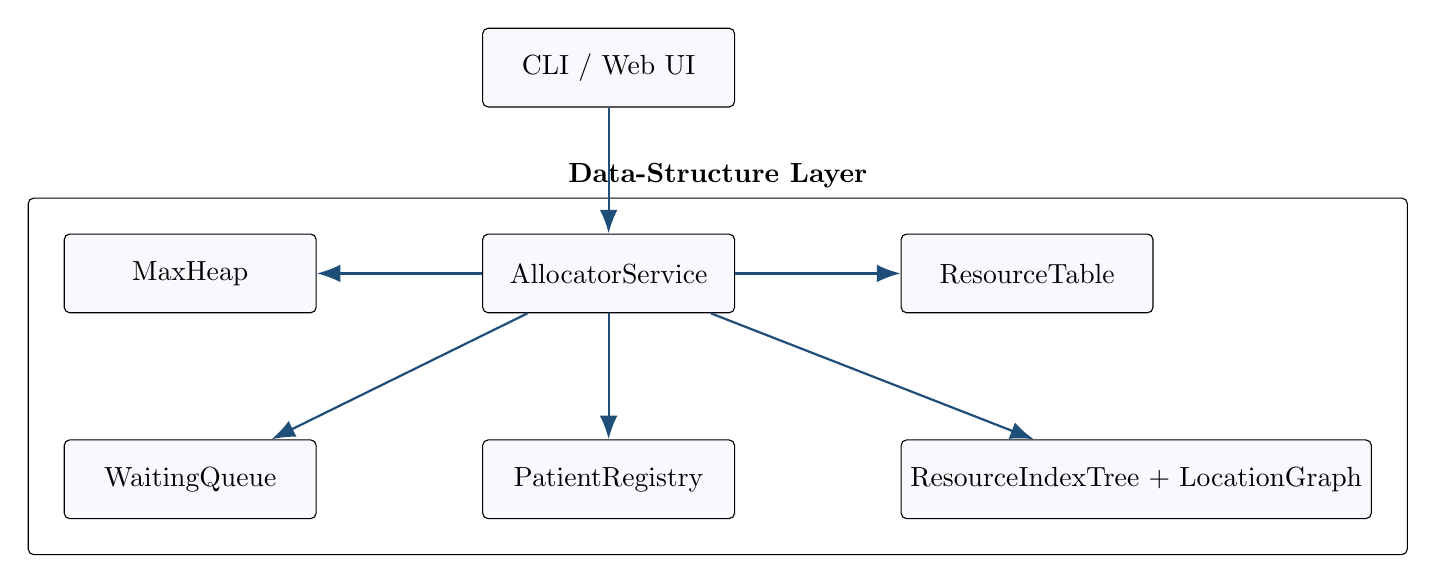
\begin{tikzpicture}[
  node distance=1.6cm and 2.1cm,
  box/.style={draw, rounded corners=2pt, fill=panel, minimum width=3.2cm, minimum height=1cm, align=center},
  arrow/.style={-{Latex[length=3mm]}, thick, color=accent}
]
\node[box] (ui) {CLI / Web UI};
\node[box, below=of ui] (service) {AllocatorService};
\node[box, left=of service] (heap) {MaxHeap};
\node[box, right=of service] (table) {ResourceTable};
\node[box, below left=of service] (queue) {WaitingQueue};
\node[box, below=of service] (registry) {PatientRegistry};
\node[box, below right=of service] (treegraph) {ResourceIndexTree + LocationGraph};
\node[draw, rounded corners=2pt, fit=(heap)(table)(queue)(registry)(treegraph), inner sep=0.45cm, label={[align=center]above:\textbf{Data-Structure Layer}}] (dsframe) {};
\draw[arrow] (ui) -- (service);
\draw[arrow] (service) -- (heap);
\draw[arrow] (service) -- (table);
\draw[arrow] (service) -- (queue);
\draw[arrow] (service) -- (registry);
\draw[arrow] (service) -- (treegraph);
\end{tikzpicture}
\caption{High-level architecture of the allocator.}
\label{fig:architecture}
\end{figure}

\section{Triage Workflow}
Figure~\ref{fig:workflow} shows the core flow used when a new emergency arrives.

\begin{figure}[H]
\centering
\begin{tikzpicture}[
  node distance=1.35cm and 1.6cm,
  every node/.style={align=center},
  step/.style={draw, rounded corners=2pt, fill=accentlight, minimum width=3.6cm, minimum height=0.95cm},
  decision/.style={draw, diamond, aspect=2.1, fill=panel, minimum width=2.3cm, inner sep=1pt},
  arrow/.style={-{Latex[length=3mm]}, thick, color=accent}
]
\node[step] (input) {Receive emergency};
\node[step, below=of input] (heap) {Insert into max-heap};
\node[step, below=of heap] (serve) {Extract top priority case};
\node[decision, below=of serve] (match) {Matching resource available?};
\node[step, below left=of match, xshift=0.55cm] (queue) {Send to waiting queue};
\node[step, below right=of match, xshift=-0.55cm] (assign) {Assign resource and record history};
\node[step, below=of assign] (route) {Suggest route and update patient registry};
\draw[arrow] (input) -- (heap);
\draw[arrow] (heap) -- (serve);
\draw[arrow] (serve) -- (match);
\draw[arrow] (match) -- node[left] {No} (queue);
\draw[arrow] (match) -- node[right] {Yes} (assign);
\draw[arrow] (assign) -- (route);
\end{tikzpicture}
\caption{Core triage flow used by the allocator.}
\label{fig:workflow}
\end{figure}

\chapter{Data Structures Used}
This project is built around several complementary structures. Each one serves a specific role and illustrates a different runtime trade-off.

\section{Max-Heap for Emergency Prioritization}
The emergency queue uses a max-heap so the highest-severity case is always at the root. If two emergencies have the same severity, arrival time is used as a tie-breaker so older cases are not starved.

\textbf{Why it fits:}
\begin{itemize}[leftmargin=1.2cm]
  \item insertion is efficient,
  \item the top-priority case is always accessible,
  \item priority updates are supported without rebuilding the entire list,
  \item the behavior is easy to explain in a viva.
\end{itemize}

\section{Hash Table for Resource Management}
Resources are indexed by ID in a hash table so lookup, assignment, and release operations remain fast on average. This is the natural structure for direct access by key.

\textbf{Used for:}
\begin{itemize}[leftmargin=1.2cm]
  \item add resource,
  \item find resource by ID,
  \item reserve a compatible resource,
  \item release a resource,
  \item count available resources.
\end{itemize}

\section{Queue for Waiting Cases}
When no compatible resource is available, the emergency is moved into a waiting queue. This preserves order and keeps unsatisfied cases from disappearing.

\section{Linked List for Patient Registry}
The patient registry stores a running record of each patient or case in insertion order. This makes it easy to keep a stable view of patient status changes, search records, and display a readable history.

\section{Binary Search Tree for Ordered Resources}
A BST provides an alternate sorted view of the resource collection. In this project, resources are shown in ordered form by resource ID, which helps demonstrate an ordered tree in addition to the hash table.

\section{Graph for Route Planning}
The location graph models roads between nodes and uses shortest-path search to suggest routes from a patient location to a compatible resource location. This adds a realistic routing dimension to the project and shows how graph traversal complements the core allocator.

\begin{figure}[H]
\centering
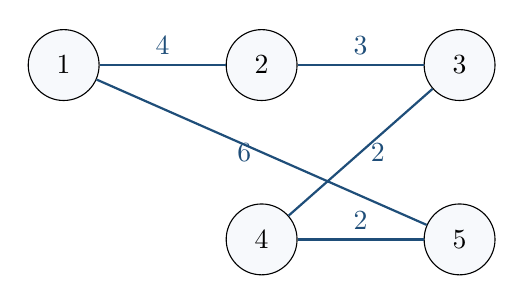
\begin{tikzpicture}[
  node distance=1.3cm and 1.6cm,
  loc/.style={draw, circle, minimum size=0.9cm, fill=panel},
  road/.style={thick, color=accent}
]
\node[loc] (n1) {1};
\node[loc, right=of n1] (n2) {2};
\node[loc, right=of n2] (n3) {3};
\node[loc, below=of n2] (n4) {4};
\node[loc, right=of n4] (n5) {5};
\draw[road] (n1) -- node[above] {4} (n2);
\draw[road] (n2) -- node[above] {3} (n3);
\draw[road] (n3) -- node[right] {2} (n4);
\draw[road] (n4) -- node[above] {2} (n5);
\draw[road] (n1) -- node[left] {6} (n5);
\end{tikzpicture}
\caption{Example location graph used by the demo scenario.}
\label{fig:graph}
\end{figure}

\chapter{Module Design}
\section{AllocatorService}
\texttt{AllocatorService} is the controller that coordinates all behavior. It receives new emergencies and resources, updates the heap, reserves resources, manages the waiting queue, refreshes patient status, stores allocation history, and computes route suggestions.

Key responsibilities include:
\begin{itemize}[leftmargin=1.2cm]
  \item inserting and updating emergencies,
  \item dispatching the next highest-priority emergency,
  \item releasing resources and retrying the waiting queue,
  \item maintaining patient records,
  \item exposing snapshot data for the UI,
  \item offering route queries for a given patient.
\end{itemize}

\section{CLI Interface}
The CLI offers a menu-based demo useful for quick viva walkthroughs. It supports core triage operations and inspection features such as patient lookup, ordered resources, and route display.

\section{Web Interface}
The web demo mirrors the backend state in a dashboard. It allows users to add emergencies, add resources, add roads, inspect patients, and request a route preview. This interface is presentation-focused and keeps the logic in C++.

\screenshotplaceholder{Insert a screenshot of the browser dashboard here, showing the live state panels.}

\chapter{Implementation Details}
\section{Emergency Handling}
An emergency is represented with severity, type, required resource type, arrival time, and location. The allocator prioritizes higher severity first and uses arrival time to preserve fairness among equal-severity cases.

\section{Resource Assignment}
When dispatching, the allocator attempts to reserve a compatible resource. If none is available, the case moves to the waiting queue. When a resource is later released or added, waiting cases are retried automatically.

\section{Patient Registry Updates}
Each emergency also creates or updates a patient record. The registry stores status transitions such as PENDING, WAITING, ASSIGNED, and COMPLETED, making the resulting report easier to inspect.

\section{Route Computation}
A route suggestion is computed only when the patient has a valid location and a compatible resource location is reachable in the graph. If the patient already has an assigned resource, the lookup can prefer that resource; otherwise it searches among compatible available resources.

\section{Demo Scenario}
The project includes a scripted demo that seeds roads, resources, emergencies, service events, and route output. The demo is useful for testing, documentation capture, and viva presentation.

\screenshotplaceholder{Insert a screenshot of the CLI demo output here, including dispatch, history, patient registry, and route information.}

\chapter{Complexity Analysis}
Table~\ref{tab:complexity} summarizes the main operations.

\begin{table}[H]
\centering
\renewcommand{\arraystretch}{1.2}
\begin{tabularx}{0.98\textwidth}{>{\bfseries}X >{\centering\arraybackslash}p{3cm} X}
\toprule
Operation & Average / Expected Cost & Notes \\
\midrule
Insert emergency into heap & $O(\log n)$ & Heapify-up preserves ordering \\
Serve next emergency & $O(\log n)$ & Extract-max then dispatch \\
Update severity & $O(\log n)$ & Reposition indexed heap item \\
Resource lookup by ID & $O(1)$ & Hash table access \\
Reserve / release resource & $O(1)$ average & Direct state mutation in hash table \\
Waiting queue push/pop & $O(1)$ & FIFO preservation \\
Patient lookup & $O(n)$ & Linked-list scan in the current design \\
Ordered resource snapshot & $O(n)$ & In-order traversal of BST \\
Shortest route search & Depends on graph size & Dijkstra-style shortest-path search \\
\bottomrule
\end{tabularx}
\caption{Complexity summary for the main operations.}
\label{tab:complexity}
\end{table}

\section{Why These Structures}
The chosen structures match the operations they support:
\begin{itemize}[leftmargin=1.2cm]
  \item heap for fast priority selection,
  \item hash table for direct resource access,
  \item queue for fairness under shortage,
  \item linked list for a simple registry of cases,
  \item BST for ordered inspection,
  \item graph for route discovery.
\end{itemize}

\chapter{Testing and Validation}
The project was validated through a combination of build checks and demo scenarios.

\section{Build Validation}
The CMake build completes successfully on Windows, which confirms that the project compiles cleanly after the current feature set.

\section{Functional Checks}
The following behaviors were verified during development:
\begin{itemize}[leftmargin=1.2cm]
  \item emergency insertion and priority ordering,
  \item severity update and heap reordering,
  \item resource assignment and release,
  \item waiting-queue retry on resource availability,
  \item patient registry population and inspection,
  \item ordered resource display,
  \item route lookup in the browser and console flows.
\end{itemize}

\section{Screenshot Placeholders}
Add final submission screenshots in these locations:
\begin{itemize}[leftmargin=1.2cm]
  \item browser dashboard after demo load,
  \item CLI output after running the scripted scenario,
  \item route preview for one selected patient,
  \item patient registry and ordered resource sections.
\end{itemize}

\chapter{Limitations and Future Work}
The project is intentionally scoped as a teaching simulator. It does not include persistence, authentication, or real hospital integrations. Future work could add:
\begin{itemize}[leftmargin=1.2cm]
  \item persistence to files or a database,
  \item multi-hospital dispatch coordination,
  \item richer route metrics and traffic-aware paths,
  \item a patient search index with faster direct lookup,
  \item analytics for average wait time and service counts.
\end{itemize}

\chapter{Conclusion}
The Emergency Resource Allocator demonstrates how multiple data structures can cooperate inside a single practical application. The max-heap handles urgency, the hash table manages resources, the queue preserves overflow cases, the linked list keeps patient records, the BST provides an ordered view, and the graph adds route planning. Together, they create a project that is both technically grounded and easy to present.

\chapter*{References}
\begin{thebibliography}{9}
\bibitem{cppref} ISO C++ reference and standard library documentation, used for language and container semantics.
\bibitem{cmake} CMake documentation, used for the build configuration and project structure.
\bibitem{algorithms} Standard data structures and algorithms course material covering heaps, hash tables, queues, trees, and graphs.
\end{thebibliography}

\appendix
\chapter{Figure and Screenshot Placeholders}
Use this appendix to paste final images before submission. Suggested file names:
\begin{itemize}[leftmargin=1.2cm]
  \item \texttt{screenshots/dashboard.png}
  \item \texttt{screenshots/cli-demo.png}
  \item \texttt{screenshots/route-preview.png}
  \item \texttt{screenshots/patient-registry.png}
\end{itemize}

\screenshotplaceholder{Insert any extra figure or screenshot here.}

\end{document}
